\begin{figure}[ht]
\caption{Agrupamientos del grafo de la lista de problemas}
\label{fig:clust_todo}
\centering
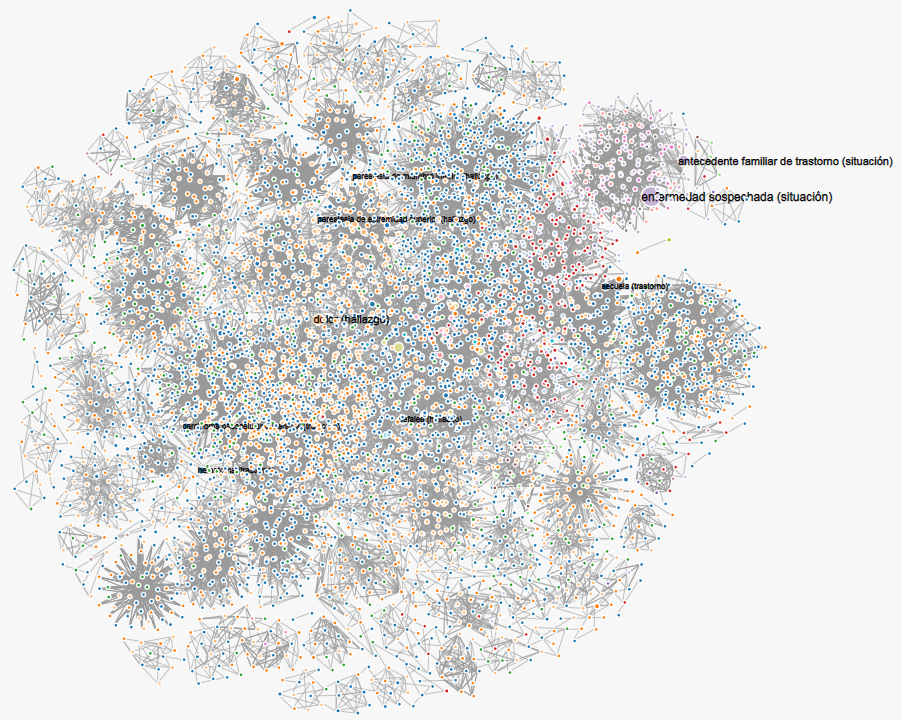
\includegraphics[width=\textwidth]{clust_todo}
\end{figure}

\begin{figure}[ht]
\caption{Agrupamientos del grafo de la lista de problemas en el contexto de los servicios de cardiología de adultos y pediátrica}
\label{fig:clust_area_cardio}
\centering
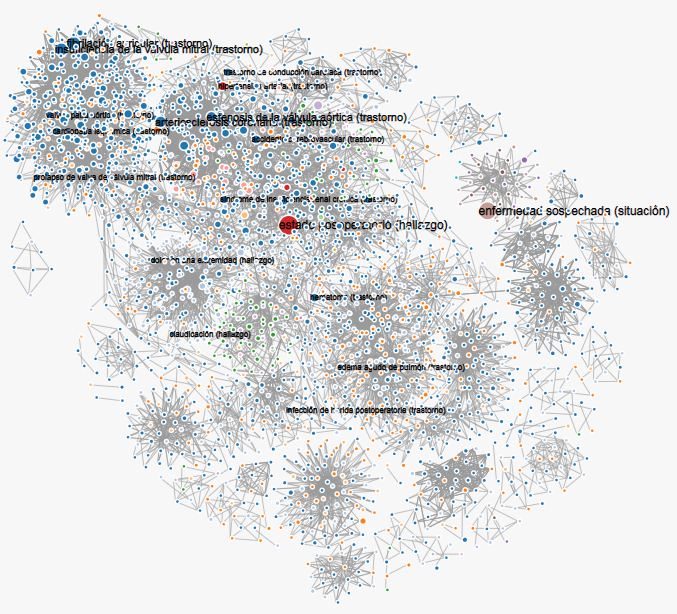
\includegraphics[width=\textwidth]{clust_area_cardio}
\end{figure}

\begin{figure}[ht]
\caption{Agrupamientos del grafo de la lista de problemas en el contexto del servicio de dermatología}
\label{fig:clust_area_dermatologia}
\centering
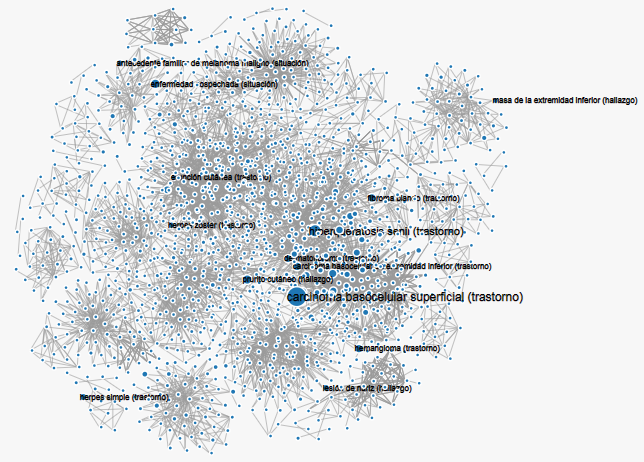
\includegraphics[width=\textwidth]{clust_area_dermatologia}
\end{figure}

\begin{figure}[ht]
\caption{Agrupamientos del grafo de la lista de problemas en el contexto de los servicios de endocrinología, nefrología y urología}
\label{fig:clust_area_ENU}
\centering
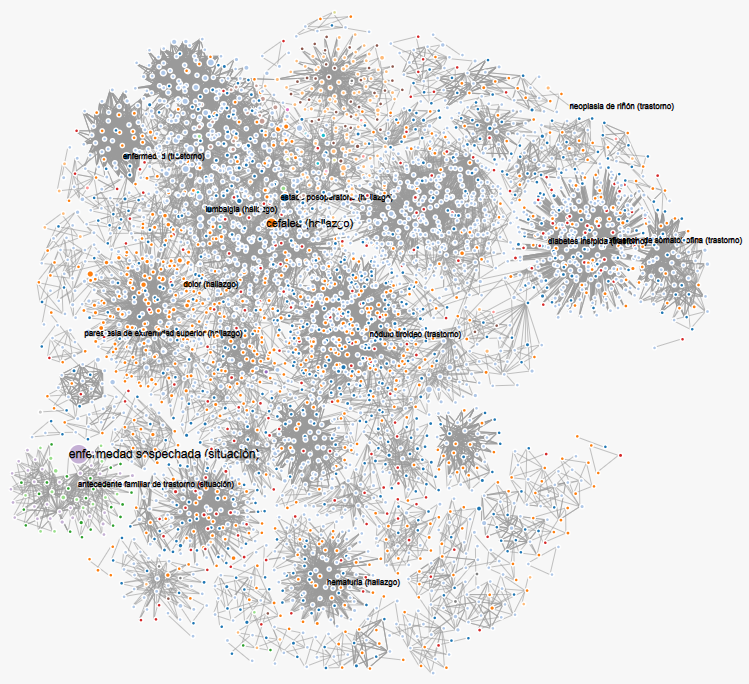
\includegraphics[width=\textwidth]{clust_area_ENU}
\end{figure}

\begin{figure}[ht]
\caption{Agrupamientos del grafo de la lista de problemas en el contexto del servicio de ginecobstreticia }
\label{fig:clust_area_gineco}
\centering
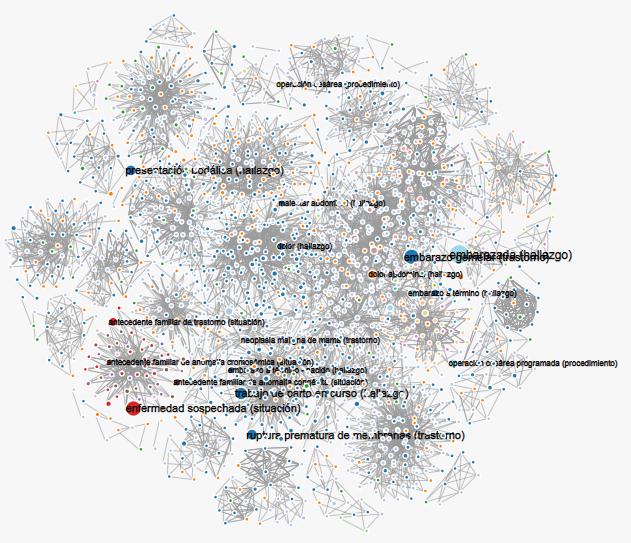
\includegraphics[width=\textwidth]{clust_area_gineco}
\end{figure}

\begin{figure}[ht]
\caption{Agrupamientos del grafo de la lista de problemas en el contexto del servicio de neurología }
\label{fig:clust_area_neuro}
\centering
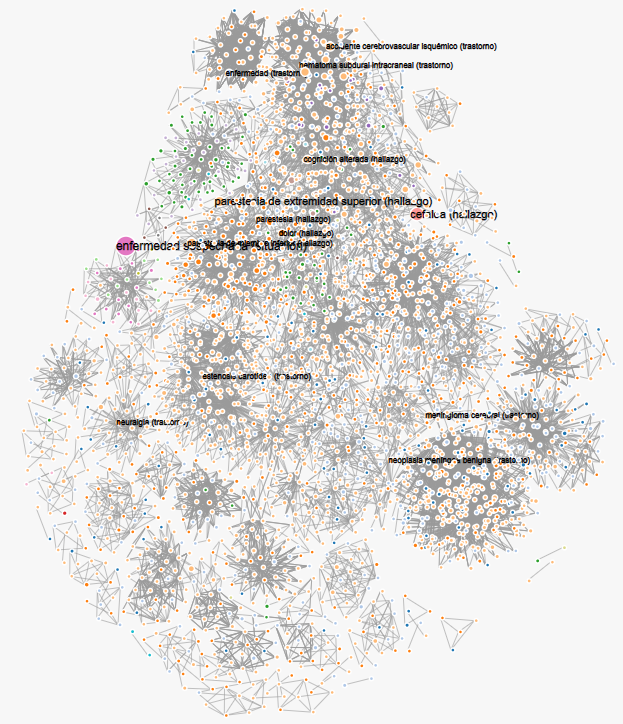
\includegraphics[width=\textwidth]{clust_area_neuro}
\end{figure}

\begin{figure}[ht]
\caption{Agrupamientos del grafo de la lista de problemas en el contexto del servicio de oftalmología }
\label{fig:clust_area_oftalmo}
\centering
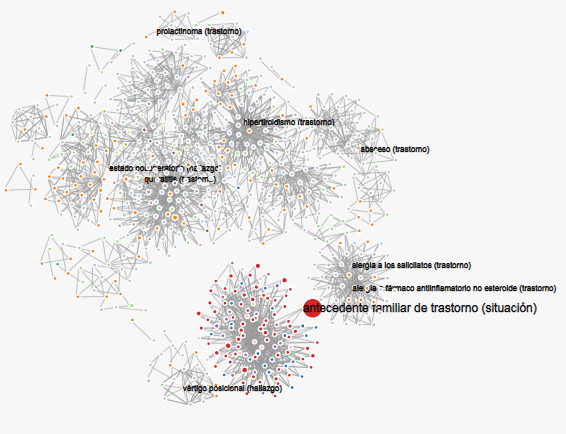
\includegraphics[width=\textwidth]{clust_area_oftalmo}
\end{figure}

\begin{figure}[ht]
\caption{Agrupamientos del grafo de la lista de problemas en el contexto del servicio de otorrinolaringología }
\label{fig:clust_area_otorrino}
\centering
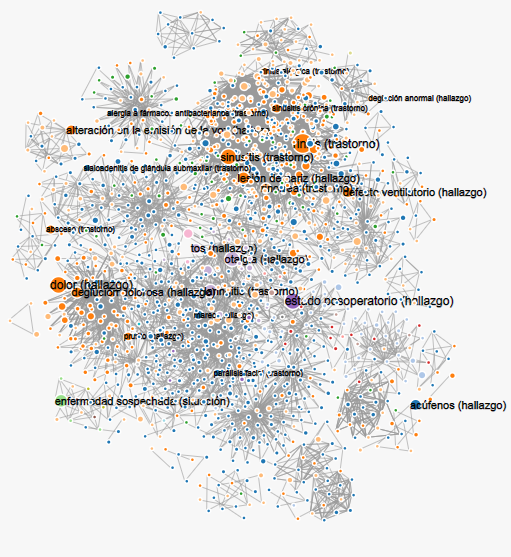
\includegraphics[width=\textwidth]{clust_area_otorrino}
\end{figure}

\begin{figure}[ht]
\caption{Agrupamientos del grafo de la lista de problemas en el contexto del servicio de pediatría }
\label{fig:clust_area_pedia}
\centering
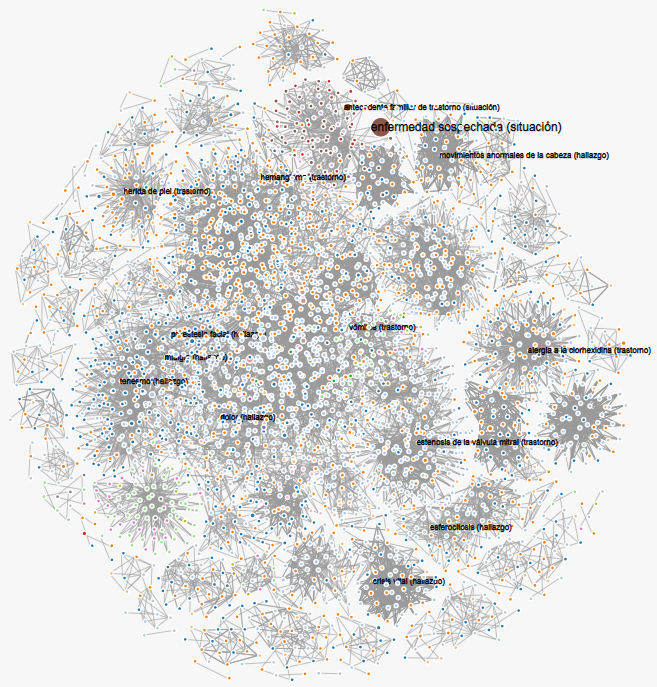
\includegraphics[width=\textwidth]{clust_area_pedia}
\end{figure}

\begin{figure}[ht]
\caption{Agrupamientos del grafo de la lista de problemas en el contexto del servicio de psiquiatría }
\label{fig:clust_area_psiqui}
\centering
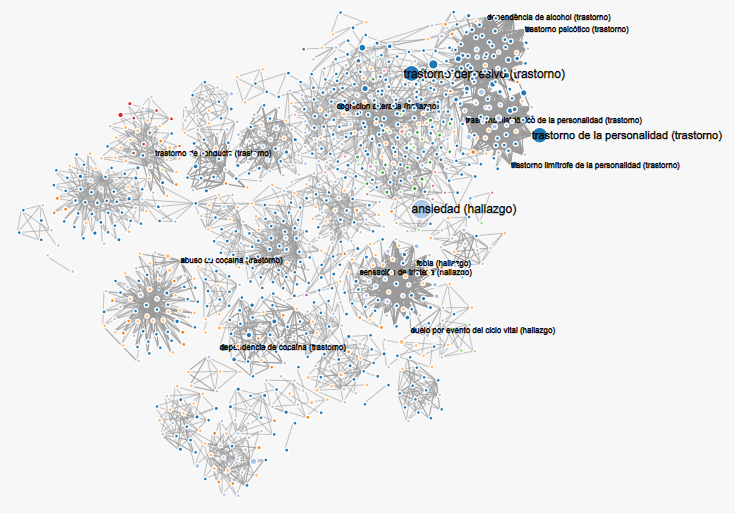
\includegraphics[width=\textwidth]{clust_area_psiqui}
\end{figure}

\begin{figure}[ht]
\caption{Agrupamientos del grafo de la lista de problemas en el contexto del servicio de traumatología }
\label{fig:clust_area_traumato}
\centering
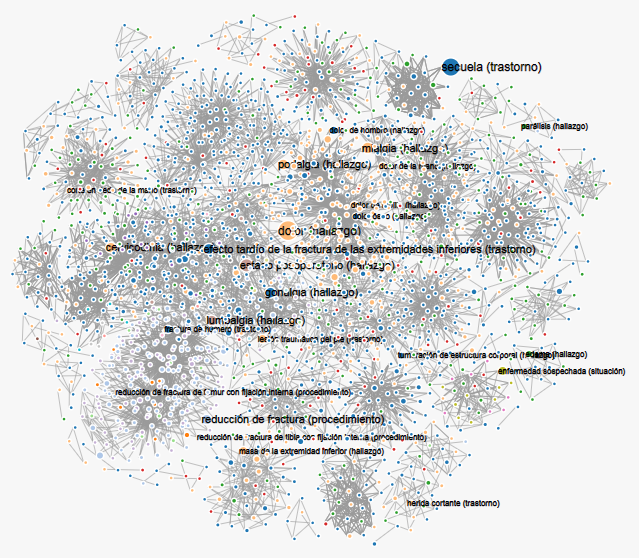
\includegraphics[width=\textwidth]{clust_area_traumato}
\end{figure}

\begin{figure}[ht]
\caption{Agrupamientos del grafo de la lista de problemas en el contexto del nivel asistencial ambulatorio }
\label{fig:clust_ambito_ambulatorio}
\centering
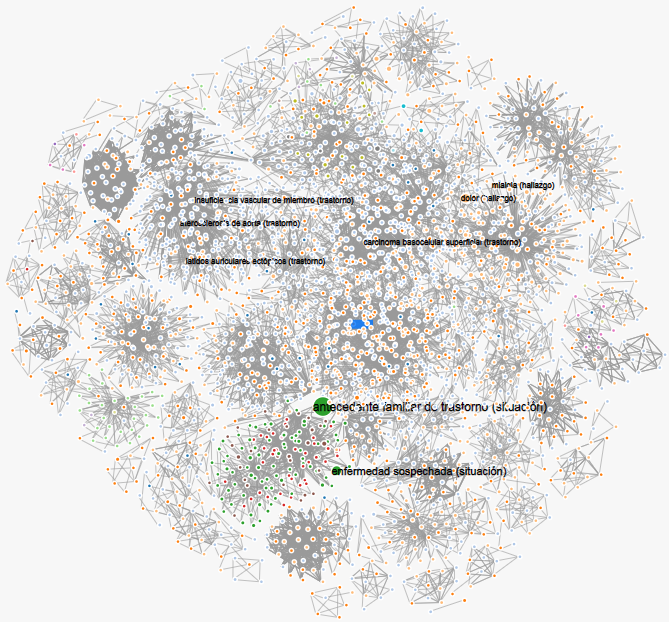
\includegraphics[width=\textwidth]{clust_ambito_1}
\end{figure}

\begin{figure}[ht]
\caption{Agrupamientos del grafo de la lista de problemas en el contexto del nivel asistencial de episodio ambulatorio }
\label{fig:clust_ambito_epi_ambulatorio}
\centering
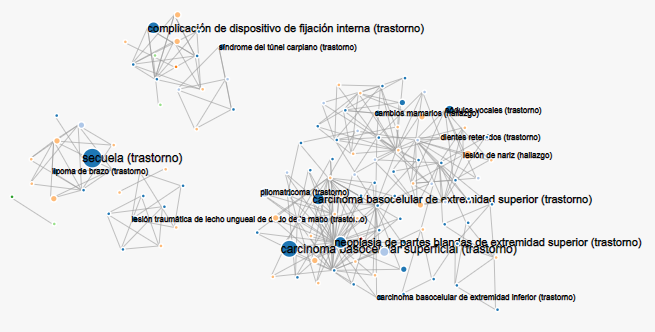
\includegraphics[width=\textwidth]{clust_ambito_9}
\end{figure}

\begin{figure}[ht]
\caption{Agrupamientos del grafo de la lista de problemas en el contexto del nivel asistencial de la guardia }
\label{fig:clust_ambito_guardia}
\centering
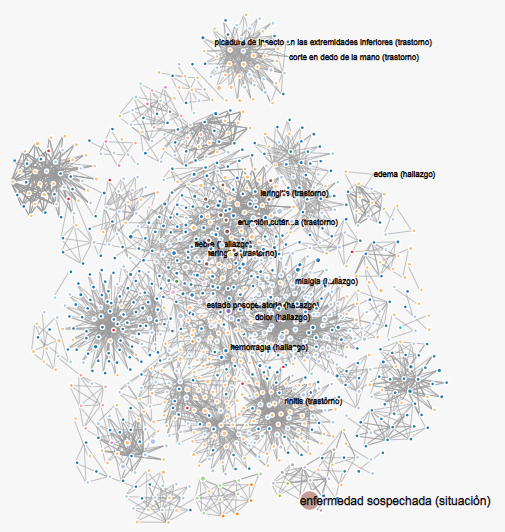
\includegraphics[width=\textwidth]{clust_ambito_3}
\end{figure}

\begin{figure}[ht]
\caption{Agrupamientos del grafo de la lista de problemas en el contexto del nivel asistencial de internación domiciliaria }
\label{fig:clust_ambito_inter_domici}
\centering
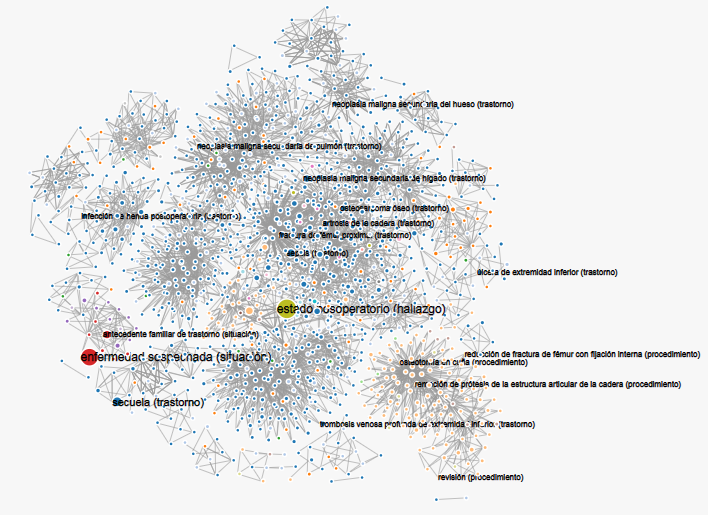
\includegraphics[width=\textwidth]{clust_ambito_6}
\end{figure}

\begin{figure}[ht]
\caption{Agrupamientos del grafo de la lista de problemas en el contexto del nivel asistencial de internación general }
\label{fig:clust_ambito_inter_general}
\centering
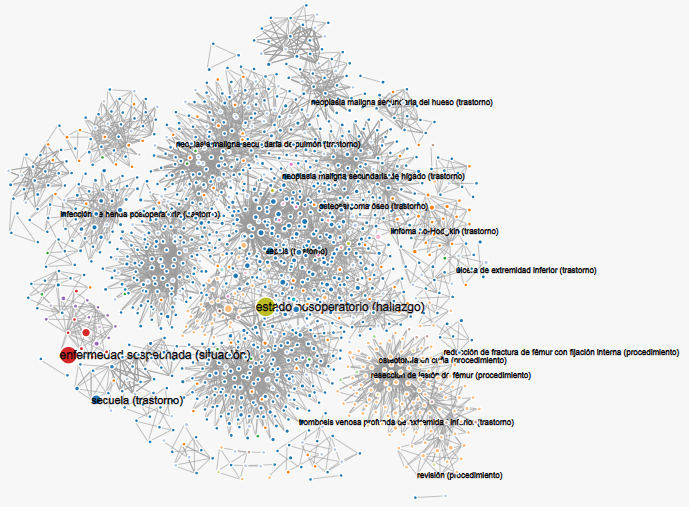
\includegraphics[width=\textwidth]{clust_ambito_2}
\end{figure}

\begin{figure}[ht]
\caption{Agrupamientos del grafo de la lista de problemas en el contexto del nivel asistencial del seguimiento domiciliario }
\label{fig:clust_ambito_segui_domici}
\centering
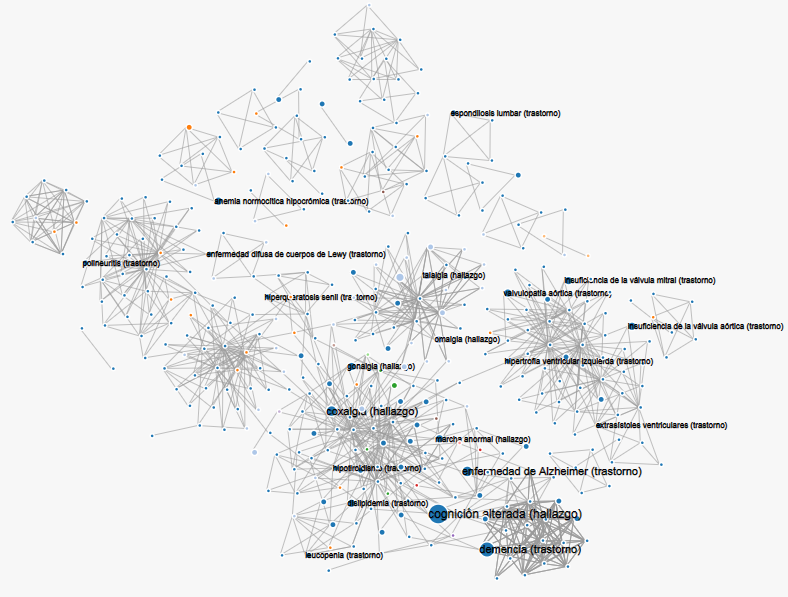
\includegraphics[width=\textwidth]{clust_ambito_7}
\end{figure}

\begin{figure}[ht]
\caption{Agrupamientos del grafo de la lista de problemas en el contexto del nivel asistencial del triage }
\label{fig:clust_ambito_triage}
\centering
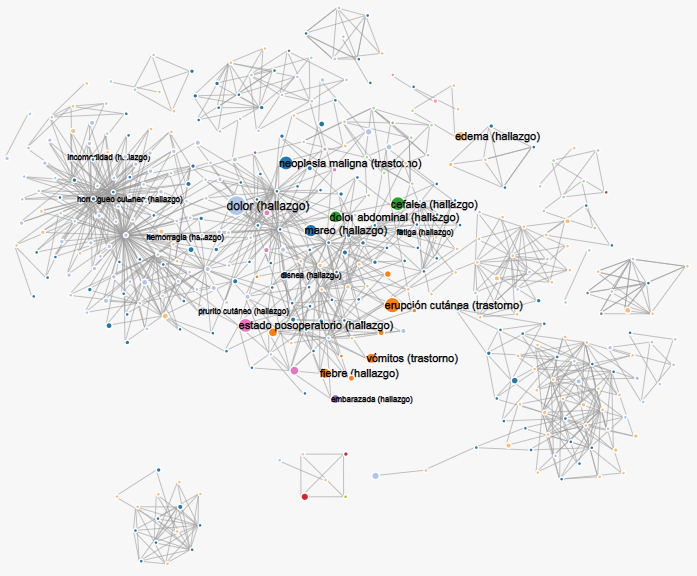
\includegraphics[width=\textwidth]{clust_ambito_4}
\end{figure}

\begin{figure}[ht]
\caption{Agrupamientos del grafo de la lista de problemas en el contexto de grupo etario de 0 a 4, 15 a 24, 25 a 34 y 35 a 44 años }
\label{fig:clust_edad_0_4}
\centering
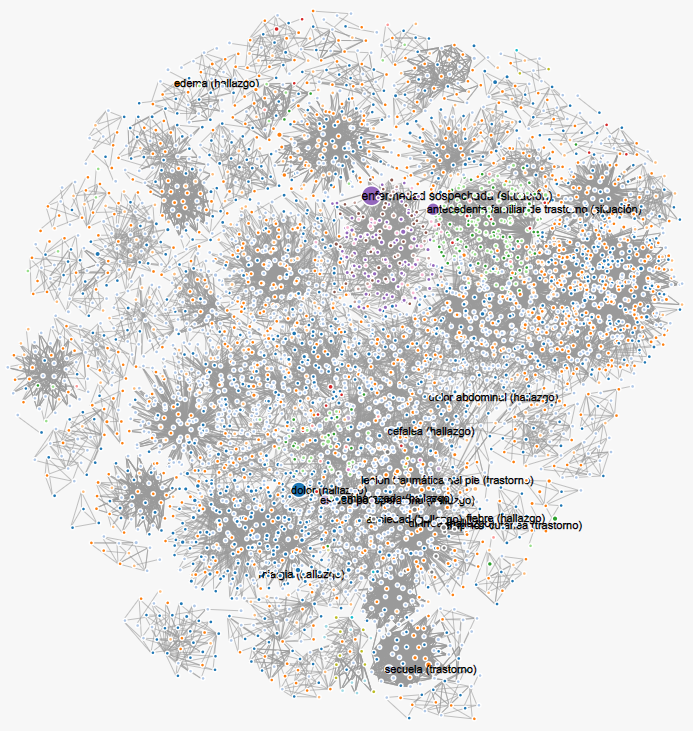
\includegraphics[width=\textwidth]{clust_edad_0-4}
\end{figure}

\begin{figure}[ht]
\caption{Agrupamientos del grafo de la lista de problemas en el contexto de grupo etario de 45 a 54 años }
\label{fig:clust_edad_45_54}
\centering
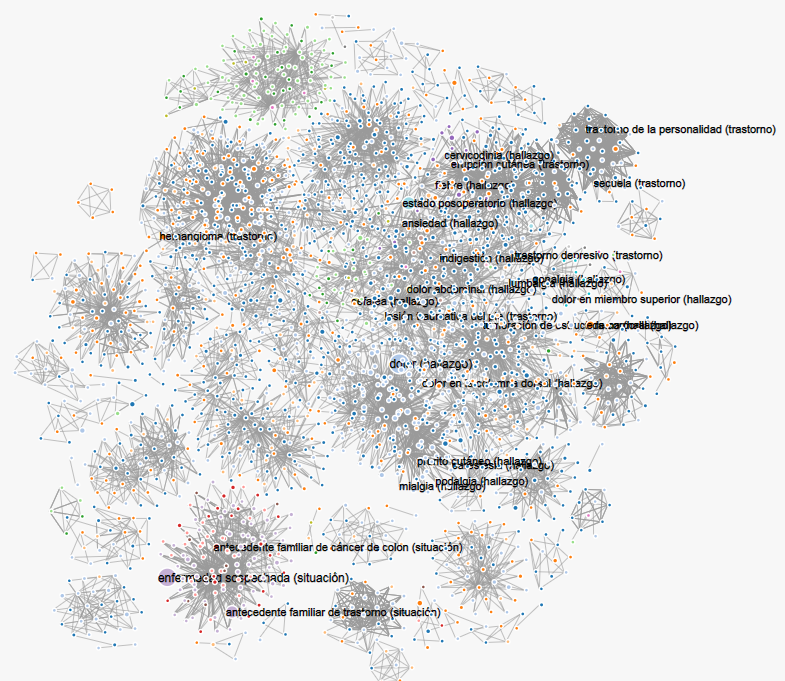
\includegraphics[width=\textwidth]{clust_edad_45-54}
\end{figure}

\begin{figure}[ht]
\caption{Agrupamientos del grafo de la lista de problemas en el contexto de grupo etario de 55 a 64 años }
\label{fig:clust_edad_55_64}
\centering
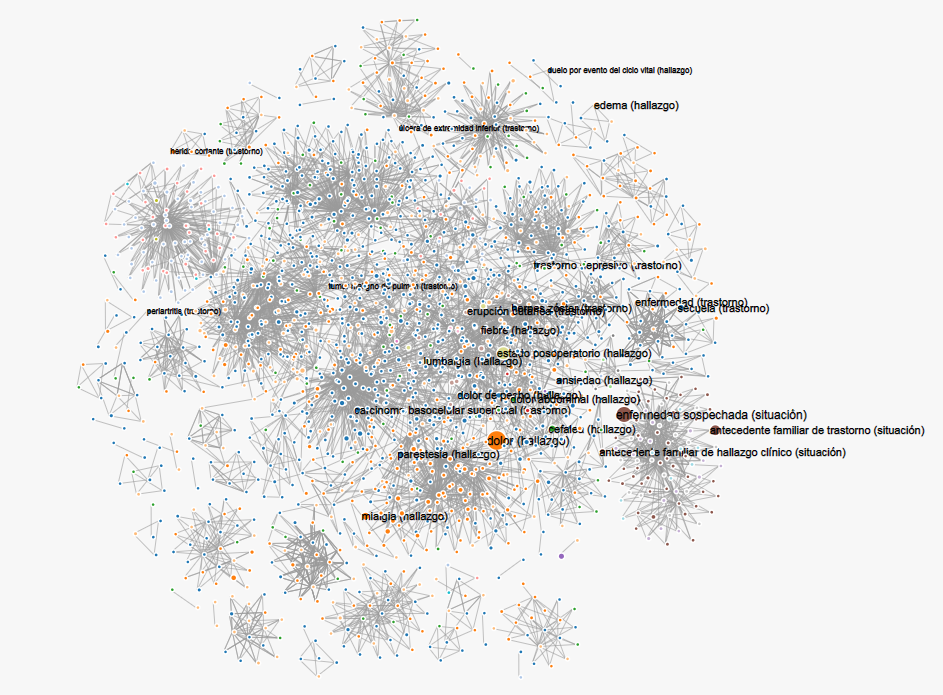
\includegraphics[width=\textwidth]{clust_edad_55-64}
\end{figure}

\begin{figure}[ht]
\caption{Agrupamientos del grafo de la lista de problemas en el contexto de grupo etario de 65 a 74 años }
\label{fig:clust_edad_65_74}
\centering
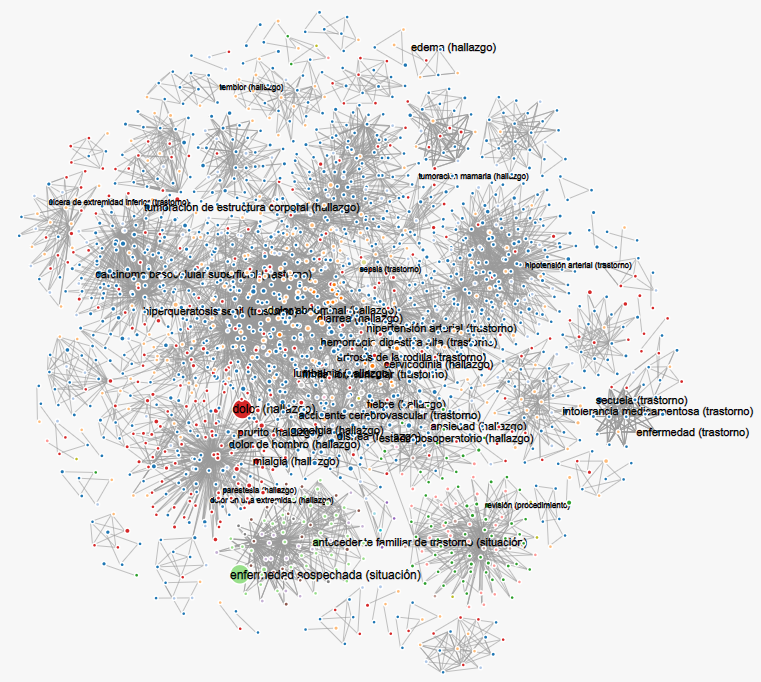
\includegraphics[width=\textwidth]{clust_edad_65-74}
\end{figure}

\begin{figure}[ht]
\caption{Agrupamientos del grafo de la lista de problemas en el contexto de grupo etario de 75 a 101 años }
\label{fig:clust_edad_75_101}
\centering
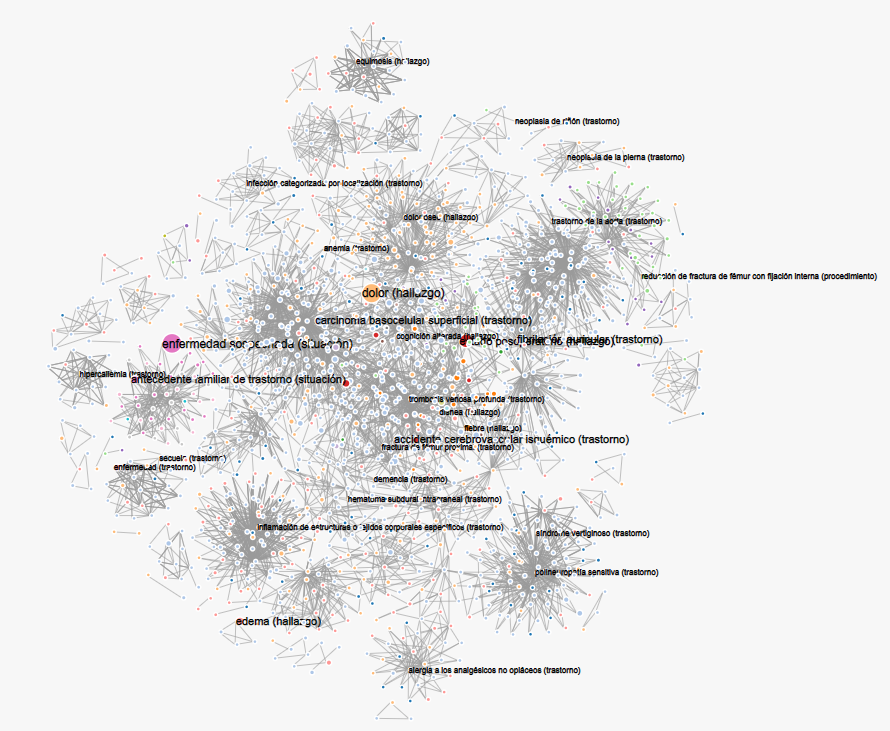
\includegraphics[width=\textwidth]{clust_edad_75-101}
\end{figure}